
\subsection{On the importance of our fixed time-encoding function.} \label{section:time_encoder}

Existing works (i.e., JODIE, TGAT, and TGN) leverage a trainable time-encoding function $\mathbf{z}(t) = \cos(t \mathbf{w}^\top + \mathbf{b})$ to represent timestamps\footnote{In fact, other baselines (e.g., CAWs, TGSRec, APAN) also utilize this trainable time-encoding function. However, we focus our discussion on the selected methods for the ease of presentation.}. 
However, we argue that using trainable time-encoding function could cause instability during training because its gradient \smash{$\frac{\partial \cos(t\mathbf{w} + \mathbf{b})}{\partial \mathbf{w}}  = t \times \sin(t\mathbf{w} + \mathbf{b})$} scales proportional to the timestamps, which could lead to training instability issue and cause the baselines' the non-smooth landscape issue as shown in Figure~\ref{fig:landscape_3d_wiki_tgat_tgn_our}. 
As an alternative, we utilize the fixed time-encoding function $\mathbf{z}(t)=\cos(t\boldsymbol{\omega})$ with fixed features $\boldsymbol{\omega}$ that could capture the relative difference between two timestamps (introduced in Section~\ref{section:method_details}).
To verify this, we introduce a simple experiment to test whether the time-encoding functions (both our fixed version and baselines' trainable version) are expressive enough, such that a simple linear classifier can distinguish the time-encodings of two different timestamps produced by the time-encoding functions. Specially, our goal is to classify if $t_1>t_2$ by learning a linear classifier on $[\mathbf{z}(t_1)~||~\mathbf{z}(t_2)]$. During training, we randomly generate two timestamps $t_1, t_2\in[0,10^6]$ and ask a fully connected layer to classify whether a timestamp is greater than another.
As shown in Figure~\ref{fig:param_trajectory_a}, using the trainable time-encoding function (orange curve) will suffer from the unstable exploding gradient issue (left upper figure) and its performance remains almost the same during the training process (left lower figure). However, using our fixed time-encoding function (blue curve) does not have the unstable exploding gradient issue and can quickly achieve high accuracy within several iterations. Meanwhile, we compare the parameter trajectories of the two models in Figure~\ref{fig:param_trajectory_b}. We observe that the change of parameters on the trainable time-encoding function is drastically larger than our fixed version. A huge change in weight parameters could deteriorate the model's performance.
Most importantly, by replacing baselines' trainable time-encoding function with our fixed version, most baselines have a smoother optimization landscape (Figure~\ref{fig:landscape_3d_fixed_time_encoder}) and a better model performance (in Table~\ref{table:average_precision_baselines_fixed_time_encoder}), which further verifies our argument that our fixed time-encoding function is more preferred than the trainable version.

\begin{figure}[h]
    \centering
    % \includegraphics[width=0.8\textwidth]{figures/param_trajectory.pdf}
    \begin{subfigure}{0.4\textwidth}
        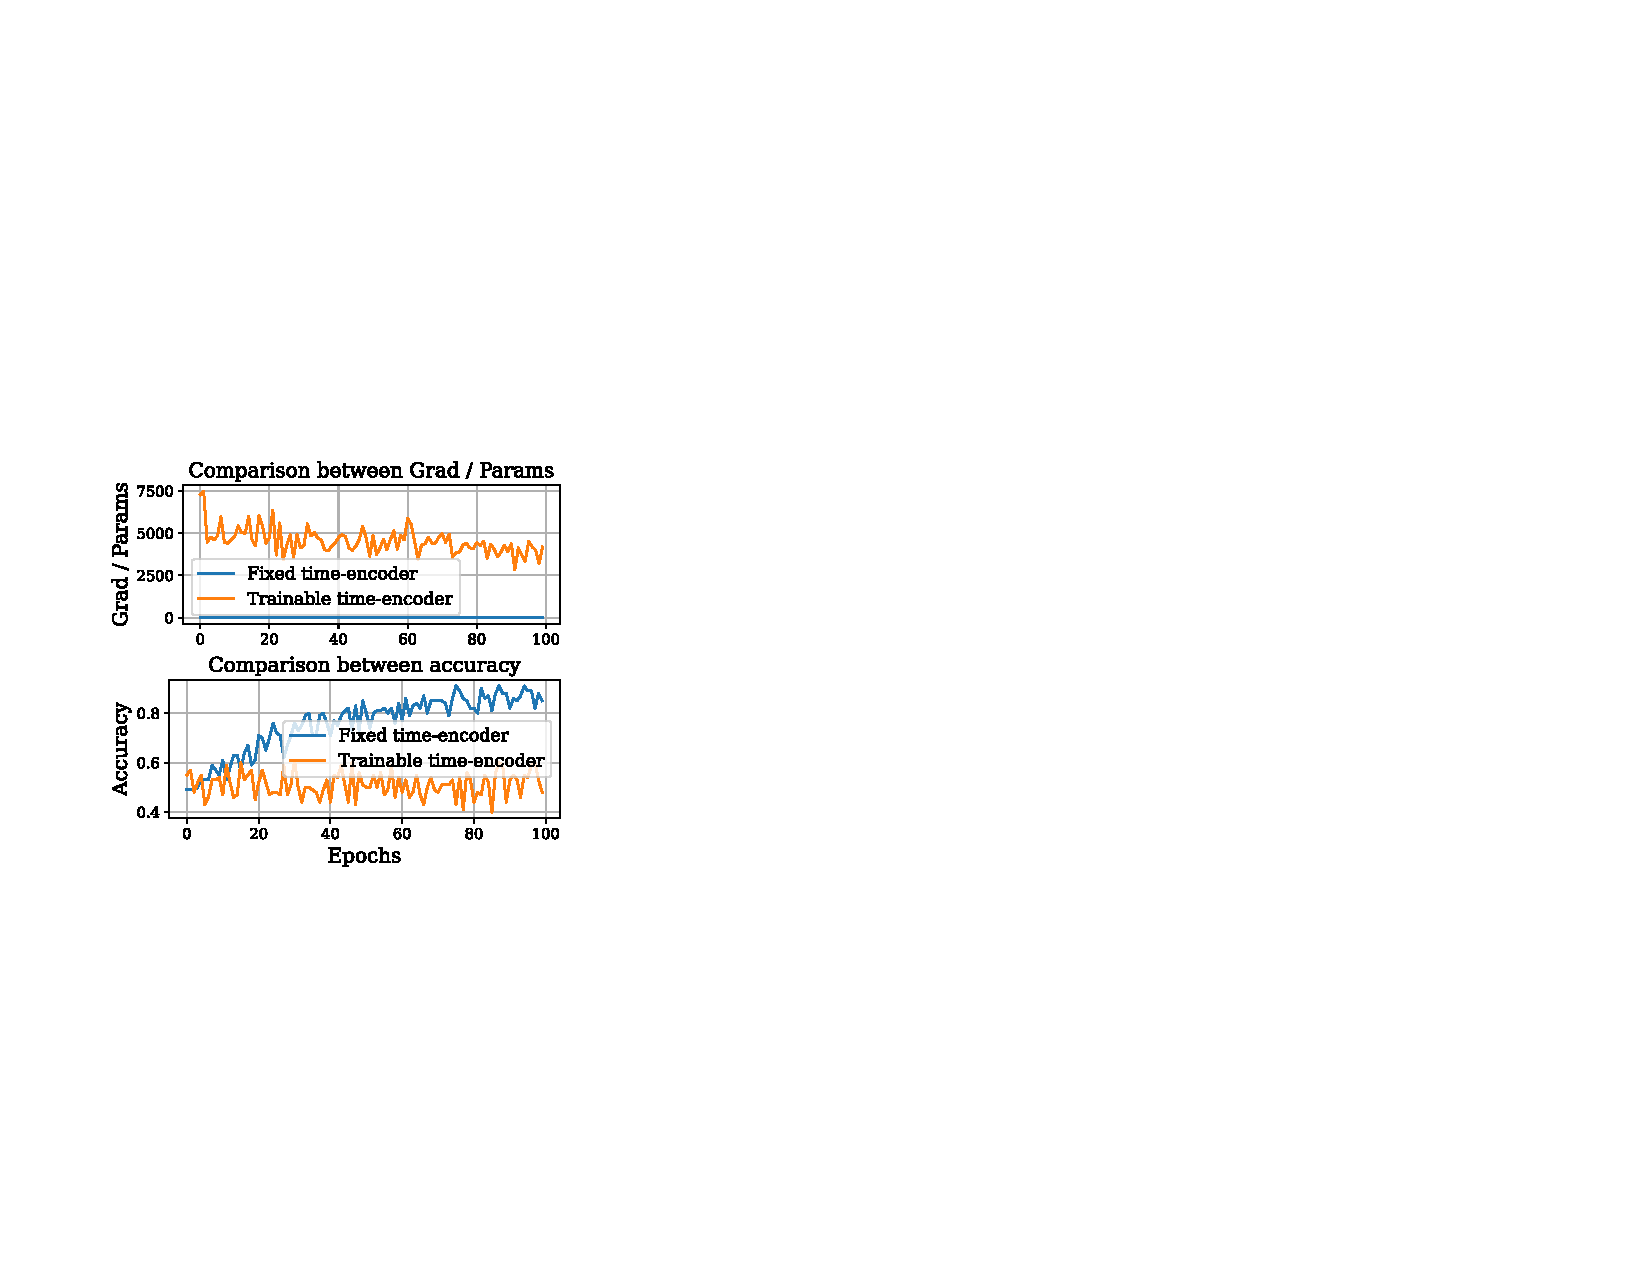
\includegraphics[width=\textwidth, height=3.9cm]{figures/param_trajectory_a.pdf}
        \vspace{-6mm}
        \caption{}
        \label{fig:param_trajectory_a}
    \end{subfigure}
    \hspace{0cm}
    \begin{subfigure}{0.4\textwidth}
        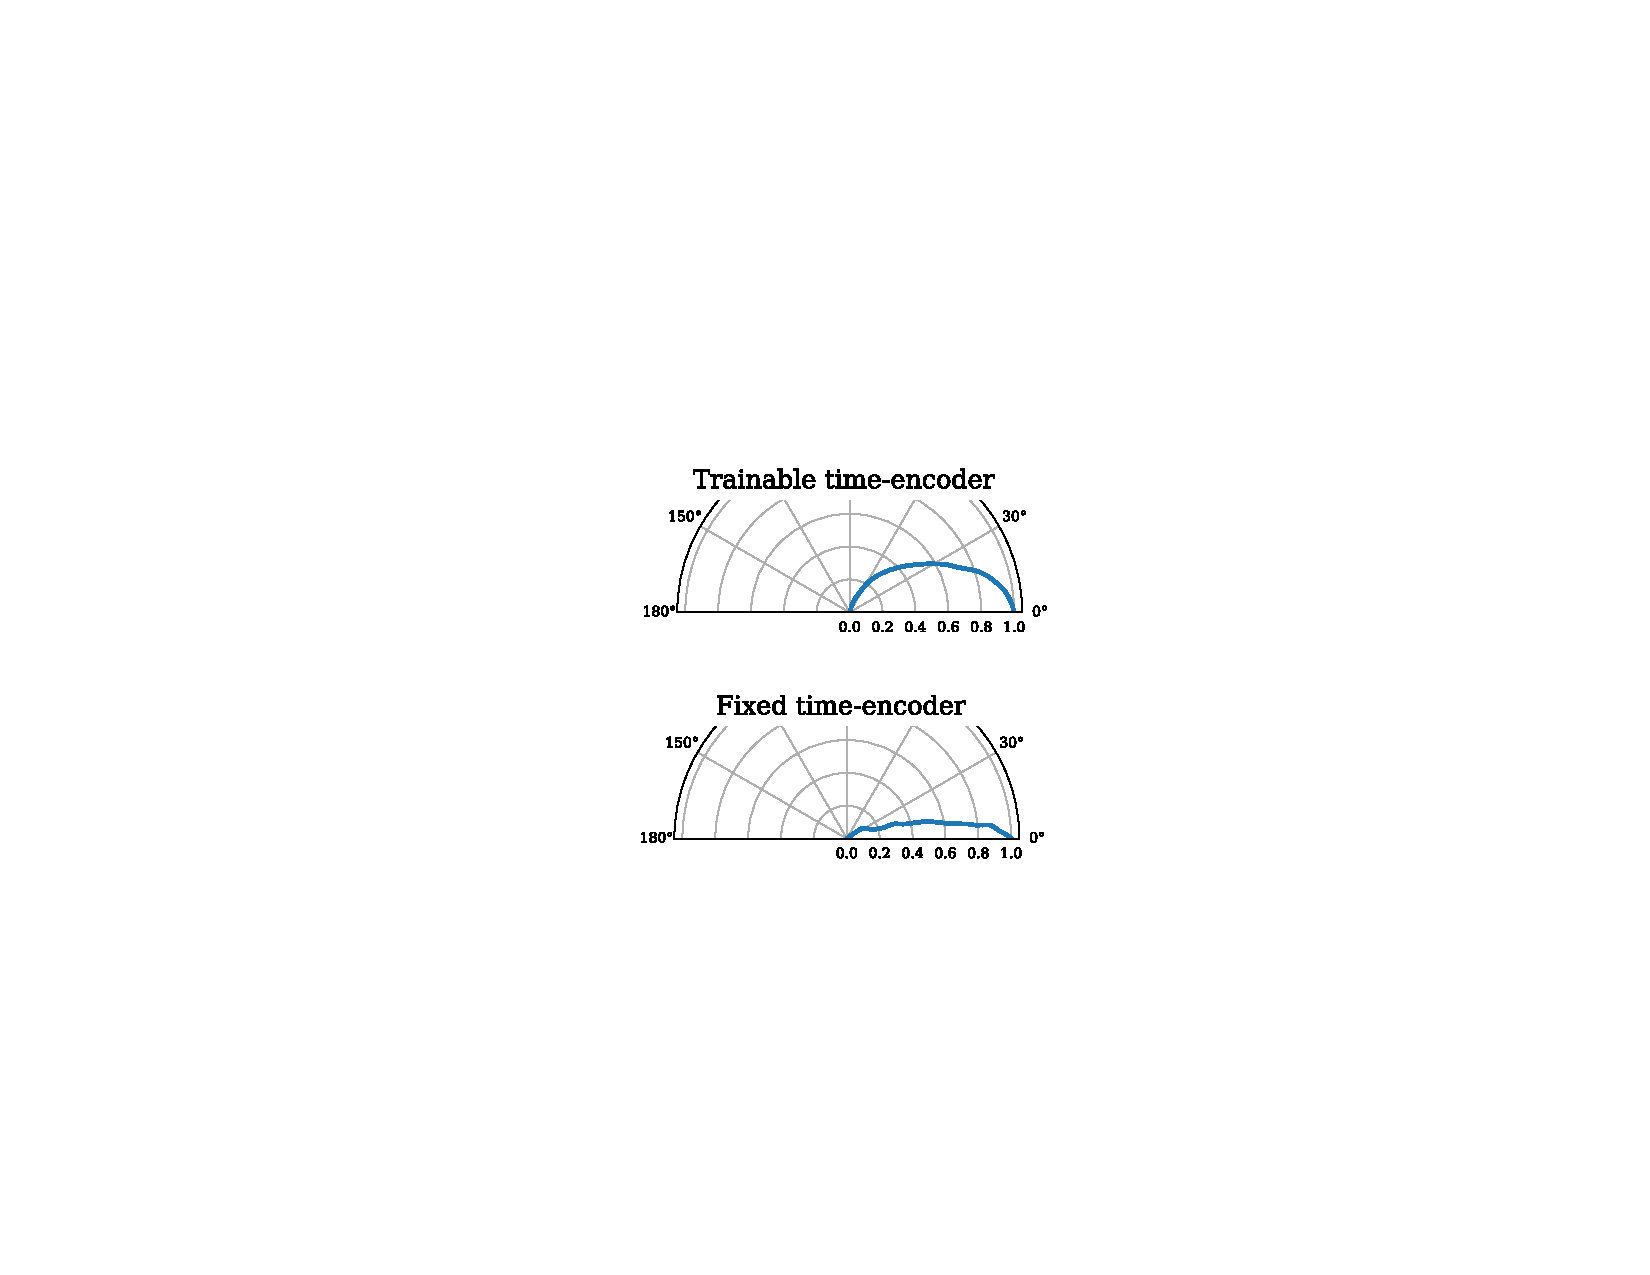
\includegraphics[width=0.9\textwidth, height=3.7cm]{figures/param_trajectory_b.pdf}
        \vspace{-3mm}
        \caption{}
        \label{fig:param_trajectory_b}
    \end{subfigure}
    \vspace{-5mm}
    \caption{(a) Comparison on the \textit{gradient / parameters norm} and \textit{accuracy} at each iteration. (b) Comparison on the trajectories of parameter change, where the radius is \smash{$r_t = \|\boldsymbol{\delta}_t\| / \|\boldsymbol{\delta}_0\|$}, the angle is \smash{$\theta_t = \arccos \langle \boldsymbol{\delta}_t / \| \boldsymbol{\delta}_t\|_2, \boldsymbol{\delta}_0 /\| \boldsymbol{\delta}_0 \|_2 \rangle$}, and \smash{$\boldsymbol{\delta}_t = \mathbf{w}_t-\mathbf{w}^\star$} is the difference between $\mathbf{w}_t$ to optimal point $\mathbf{w}^\star$. The more the model parameters change during training, the larger the semicircle.}
    \label{fig:param_trajectory}
    \vspace{-2mm}

\end{figure}


\begin{figure}[h]
\centering
\begin{subfigure}{0.24\textwidth}
    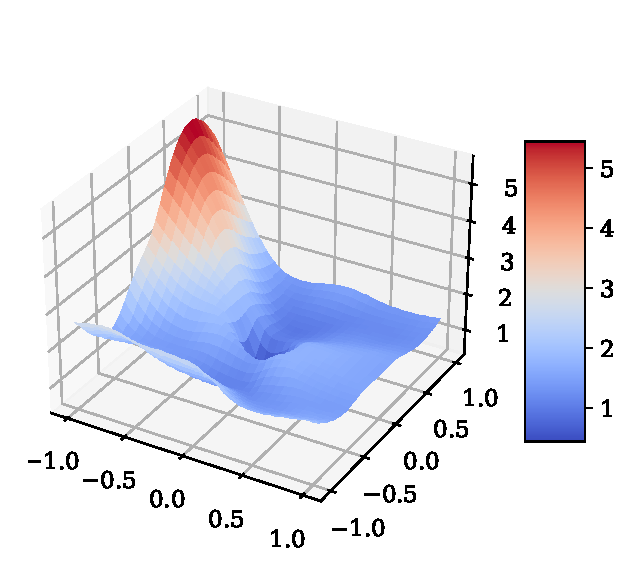
\includegraphics[width=\textwidth,height=2.3cm]{figures/fixed_time_encoding_main_text/gdelt_lite_landscape_gdelt_lite_tgat_surf_file.h5_train_loss_3dsurface.pdf}
    \vspace{-6mm}
    \caption{TGAT on GDELT-e}
\end{subfigure}
\hspace{0cm}
\begin{subfigure}{0.24\textwidth}
    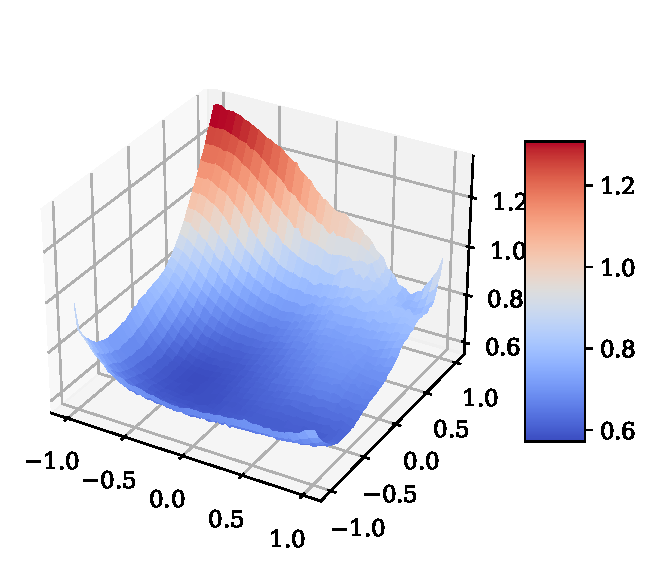
\includegraphics[width=\textwidth,height=2.3cm]{figures/fixed_time_encoding_main_text/gdelt_lite_landscape_gdelt_lite_tgn_surf_file.h5_train_loss_3dsurface.pdf}
    \vspace{-6mm}
    \caption{TGN on GDELT-e}
\end{subfigure}
\hspace{0cm}
\begin{subfigure}{0.24\textwidth}
    
\includegraphics[width=\textwidth,height=2.3cm]{figures/fixed_time_encoding_main_text/wiki_landscape_wiki_tgat_surf_file.h5_train_loss_3dsurface.pdf}
    \vspace{-6mm}
    \caption{TGAT on Wiki}
\end{subfigure}
\hspace{0cm}
\begin{subfigure}{0.24\textwidth}
    
\includegraphics[width=\textwidth,height=2.3cm]{figures/fixed_time_encoding_main_text/wiki_landscape_wiki_tgn_surf_file.h5_train_loss_3dsurface.pdf}
    \vspace{-6mm}
    \caption{TGN on Wiki}
\end{subfigure}
\vspace{-4mm}
\caption{Comparison on the training loss landscape \textit{fixed time-encoding function}. Results on other datasets and baselines can be found in Appendix~\ref{section:loss_landscape_appendix_fixed_time_encoder}. }
\label{fig:landscape_3d_fixed_time_encoder}
\vspace{-4mm}

\end{figure}

% \begin{table}[h]
% \caption{Comparison baseline with fixed time encoder (denoted as ``+fte''). Please refer to Table~\ref{table:average_precision} to compare with its average precision score with trainable time encoder.} % and  Hits$@$K 
% \label{table:average_precision_baselines_fixed_time_encoder}
% \vspace{-3mm}
% \centering
% \scalebox{0.8}{
% \begin{tabular}{ l  c c  c  c c c }
% \hline\hline
%       & Reddit & Wiki & MOOC & LastFM  & GDELT-ne & GDELT-e \\ \hline\hline
% JODIE+fte   & 99.76 & 99.00 & 99.17 & 0.7989 & 98.23 & 96.96    \\ 
% TGAT+fte    & 99.48 & 98.55 & 99.33 & 0.7626 & 92.31 & 96.28    \\
% TGN+fte     & 99.83 & 99.54 & 99.62 & 0.8758 & 98.25 & 97.34    \\ 
% \hline\hline
% \end{tabular}}
% \vspace{-2mm}
% \end{table}

\begin{table}[h]
\caption{Comparison on average precision score with fixed/trainable time encoding function (TEF).
The results before ``$\rightarrow$'' is for trainable TEF (same as Table~\ref{table:average_precision}) and after ``$\rightarrow$'' is for fixed TEF.} % and  Hits$@$K 
\label{table:average_precision_baselines_fixed_time_encoder}
\vspace{-3mm}
\centering
\scalebox{0.8}{
\begin{tabular}{ l  c c  c  c c c }
\hline\hline
       & Reddit & Wiki & MOOC & LastFM  & GDELT-ne & GDELT-e \\ \hline\hline
JODIE   & $99.30 \rightarrow \mathbf{99.76}$ & $98.81\rightarrow \mathbf{99.00}$ & $99.16\rightarrow\mathbf{99.17}$ & $67.51\rightarrow\mathbf{79.89}$ & $97.13\rightarrow\mathbf{98.23}$ & $96.96\rightarrow\mathbf{96.96}$    \\ 
TGAT    & $98.66\rightarrow\mathbf{99.48}$ & $96.71\rightarrow\mathbf{98.55}$ & $98.43\rightarrow\mathbf{99.33}$ & $54.77\rightarrow\mathbf{76.26}$ & $84.30\rightarrow\mathbf{92.31}$ & $\mathbf{96.96}\rightarrow96.28$    \\
TGN     & $99.80\rightarrow\mathbf{99.83}$ & $\mathbf{99.55}\rightarrow99.54$ & $99.62\rightarrow\mathbf{99.62}$ & $82.23\rightarrow\mathbf{87.58}$ & $98.15\rightarrow\mathbf{98.25}$ & $96.04\rightarrow\mathbf{97.34}$    \\ 
\hline\hline
\end{tabular}}
\vspace{-3mm}
\end{table}

% \weilin{although we are just comparing the selection of most representative baselines, we would like to note that CAWs, TGSRec, APAN, DDGCL also utilize a trainable time-encoding function.}

\subsection{On the importance of MLP-mixer in \oure's link-encoder} \label{section:expressive_power}

In this section, we aim to achieve a deeper understanding on the expressive power of the link-encoder by answering the following two questions: ``\textit{Can we replace the MLP-mixer in link-encoder with self-attention}?'' and ``\textit{Why MLP-mixer is a good alternative of self-attention?}''
To answer these questions, let us first conduct experiments by replacing the MLP-mixer in link-encoder with full/1-hop self-attention and sum/mean-pooling, where full self-attention is widely used in Transformers and 1-hop self-attention is widely used in graph attention networks. As shown in Table~\ref{table:average_precision_mixer_vs_attention}, \our suffers from performance degradation when using self-attention: the best performance is achieved when using MLP-mixer with zero-padding, while the model performance drop slightly when using self-attention with sum-pooling (row 2 and 4), and the performance drop significantly when using self-attention with mean-pooling (row 3 and 5). 
Self-attention with mean-pooling has a  weaker model performance because it cannot distinguish ``temporal sequences with identical link timestamps and features'' (e.g., cannot distinguish $[a_1, a_1]$ and $[a_1]$
% \footnote{We use $a_i\triangleq(t_i,\mathbf{x}_{e_i})$ to represent the combination of timestamp and feature information of link $e_i$.}) 
and it cannot explicitly capture ``the length of temporal sequences'' (e.g., cannot distinguish if $[a_1, a_2]$ is longer than $[a_3]$), which are both very important for \our understand how frequent a node interacts with other nodes.
We explicitly verify this in Figure~\ref{fig:length_cls} by first generating two temporal sequences (with timestamps but without link features), then encoding the timestamps into vectors via time-encoding function, and asking full self-attention and MLP-mixer to distinguish.
As shown in Figure~\ref{fig:length_cls}, self-attention with mean-pooling cannot distinguish two temporal sequences with identical timestamps  (because all the self-attention weights are equivalent if the features of the node on the two sides of a link are identical) and cannot capture the sequence length (because of mean-pooling simply averages the inputs and does not take the input size into consideration).
However, MLP-mixer in \our can distinguish the above two sequences because of zero-padding.
Fortunately, the aforementioned two weaknesses could be alleviated by replacing the mean-pooling in temporal self-attention with the sum-pooling, which explains why using sum-pooling brings better model performance than mean-pooling.
However, since self-attention modules have more parameters and are harder to train, they could generalize poor when the downstream task is not too complicated.


\begin{table}[t]
\caption{Comparison on the average precision score. $\natural$ use $20$ neighbors due to out of GPU memory.} % and  Hits$@$K 
\label{table:average_precision_mixer_vs_attention}
\vspace{-4mm}
\centering
\centering\setlength{\tabcolsep}{3.7mm}
\scalebox{0.85}{
\begin{tabular}{ l l  cc cc c }
\hline\hline
Link-info encoder with       & & Reddit & Wiki & MOOC & LastFM & GDELT-ne \\ \hline\hline
(Default) MLP-mixer   & + Zero-padding & $\mathbf{99.93}$ & $\textbf{99.85}$ & $\textbf{99.91}$ &  $\textbf{96.31}$ & $\textbf{98.39}$ \\ \hline
\multirow{2}{*}{Full self-attention} & + Sum pooling & $99.81$ & $98.19$ & $99.55$ & $93.97$ & $98.28^\natural$ \\ 
 & + Mean pooling& $99.00$ & $98.05$ & $99.31$ & $89.15$ & $97.13^\natural$ \\ \hline
\multirow{2}{*}{1-hop self-attention} & + Sum pooling& $99.81$ & $98.01$ & $99.30$ & $93.69$ & $98.16$ \\ 
 & + Mean pooling& $98.94$ & $97.29$ & $98.96$ & $72.32$ & $97.09$ \\ 
\hline
\end{tabular}}
\vspace{-3mm}
\end{table}


\begin{figure}[t]
\centering
\begin{subfigure}{0.45\textwidth}
    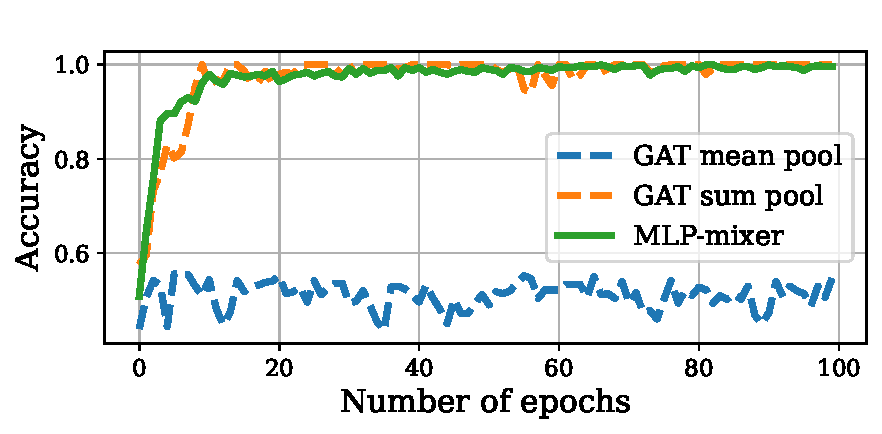
\includegraphics[width=\textwidth,height=0.35\textwidth]{figures/length_cls/length_cls_all_one.pdf}
    \vspace{-6mm}
    \caption{e.g., classify if $[a_1, a_1] = [a_1]$}\label{fig:length_cls_all_one}
\end{subfigure}
\hspace{0cm}
\begin{subfigure}{0.45\textwidth}
    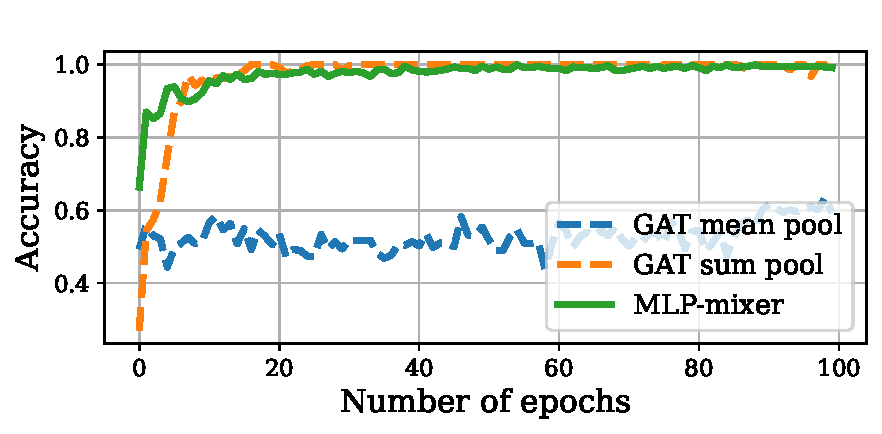
\includegraphics[width=\textwidth,height=0.35\textwidth]{figures/length_cls/length_cls_rand.pdf}
    \vspace{-6mm}
    \caption{e.g., classify if $\text{size}[a_1, a_2] > \text{size}[a_3]$} \label{fig:length_cls_rand}
\end{subfigure}
\vspace{-3mm}
\caption{(a) We generate identical timestamp sequences with different length, then ask MLP-mixer and GAT to distinguish whether the generated sequence are identical (b) We generate random sequence with different length, then ask MLP-mixer and GAT to classify which sequence is longer.}
\label{fig:length_cls}
\vspace{-5mm}

\end{figure}



% To see this, let us suppose we are aggregating information to the first item in each sequence, then the message on $\text{}\mathcal{S}_1$ is computed as
% \begin{equation*}
%     \sum_{t^\prime \in \mathcal{S}_1} \frac{\text{attn}(\mathbf{z}(t_1), \mathbf{z}(t^\prime)) \times \mathbf{z}(t_j)}{\sum_{t^\prime \in \mathcal{S}_1} \text{attn}(\mathbf{z}(t_1), \mathbf{z}(t^\prime))} = \sum_{t^\prime \in \mathcal{S}_2} \frac{\text{attn}(\mathbf{z}(t_1), \mathbf{z}(t^\prime)) \times \mathbf{z}(t_j)}{\sum_{t^\prime \in \mathcal{S}_2} \text{attn}(\mathbf{z}(t_1), \mathbf{z}(t^\prime))}
% \end{equation*}



% \weilin{if using trainable time-encoding function + sum pooling --> uniform approximate but suffer training instability issue; if using fixed time-encoding function, then it cannot uniform approximate ...}




% 1-hop self-attention with mean-pooling (marked as $\natural$) can be think of as a variant of TGAT with 1-hop recent neighbor sampling with our fixed time-encoding function.

\subsection{Key factors to the better performance} \label{section:data_alignment}


One of the major factors that contributes to \oure's success is the simplicity of \oure's neural architecture and input data.
Using conceptually simple input data that better aligned with their labels allows a simple neural network model to capture the underlying mapping between the input to their labels, which could lead to a better generalization ability.
In the following, we explicitly verify this by comparing the performance of \our with different input data in Table~\ref{table:average_precision_input_data_quality}: 
\circled{1} Recall from Section~\ref{section:some_differences} that the ``most recent 1-hop neighbors'' sampled for the two nodes on the ``undirected'' temporal graph could provide information on whether two nodes are frequently connected in the last few timestamps, which is essential for temporal graph link prediction. To verify this, we conduct ablation study by comparing the model performance on direct and undirected temporal graphs. As shown in the 1st and 2nd row of Table~\ref{table:average_precision_input_data_quality},  changing from undirected to direct graph results in a significant performance drop because such information is missing.
% \footnote{Changing to undirected graph on baseline methods does not improve their performance because they capture such information through the neural architecture design or other node sampled strategies. See Appendix~\ref{section:baseline_undirected}.}
\circled{2} Recall from Section~\ref{section:method_details} that instead of feeding the raw timestamp to \our and encoding each timestamp with a trainable time-encoding function, \our encodes the timestamps via our fixed time-encoding function and feed the encoded representation to \oure, which reduces the model complexity of learning a time-encoding function from data. 
This could be verified by the 3rd and 4th rows of Table~\ref{table:average_precision_input_data_quality}, where using the pre-encoded time information could give us a better performance.
\circled{3} Selecting the input data that has similar distribution in training and evaluation set could also potentially improve the evaluation error. For example, using  relative timestamps (i.e., each neighbor's timestamp is subtracted by its root node's timestamp) is better than absolute timestamps (e.g., using Unix timestamp)because the absolute timestamps in the evaluation set and training set are from different range when using chronological splits, but they are very likely to overlap if using relative timestamps.
As shown in the 3rd to 6th rows of Table~\ref{table:average_precision_input_data_quality}, using relative time information always gives a better model performance than using absolute time information.
\circled{4} Selecting the most representative neighbors for each node. For example, we found 1-hop most recent interacted neighbors are the most representative for link prediction. Switching to either 2-hop neighbors or uniform sampled neighbors will hurt the model performance according to the 7th to the 10th row of Table~\ref{table:average_precision_input_data_quality}.

\begin{table}[h]
\caption{Comparison on the average precision score of \our with different input data. The highlighted rows are identical to our default setting.
} % and  Hits$@$K 
\label{table:average_precision_input_data_quality}
\vspace{-3mm}
\centering
\centering\setlength{\tabcolsep}{3.5mm}
\scalebox{0.85}{
\begin{tabular}{ l rr  ll ll }
\hline\hline
  & & & Reddit & Wiki & MOOC & LastFM \\ \hline\hline
\multirow{2}{*}{\begin{tabular}[c]{@{}l@{}} Direct vs undirect \\ temporal graph \end{tabular}}       & \multicolumn{2}{r}{Directed temporal graph} & $99.69$ & $88.37$ &  $97.87$ & $78.34$           \\
                                                                              & \multicolumn{2}{r}{\cellcolor[HTML]{FEDEDC}Undirected temporal graph} & \cellcolor[HTML]{FEDEDC}$\mathbf{99.93}$ & \cellcolor[HTML]{FEDEDC}$\mathbf{99.85}$ & \cellcolor[HTML]{FEDEDC}$\mathbf{99.91}$ &  \cellcolor[HTML]{FEDEDC}$\mathbf{96.31}$  \\ \hline
\multirow{4}{*}{\begin{tabular}[c]{@{}l@{}}Time\\ information\end{tabular}}       & \multicolumn{2}{r}{Relative timestamp $(t_i-t_0)$} & $99.79$ & $99.80$ &  $99.81$ & $95.32$           \\
                                                                              & \multicolumn{2}{r}{\cellcolor[HTML]{FEDEDC}Relative time-encoding $\cos((t_i-t_0)\boldsymbol{\omega})$} & \cellcolor[HTML]{FEDEDC}$\mathbf{99.93}$ & \cellcolor[HTML]{FEDEDC}$\mathbf{99.85}$ & \cellcolor[HTML]{FEDEDC}$\mathbf{99.91}$ &  \cellcolor[HTML]{FEDEDC}$\mathbf{96.31}$  \\
                                                                              & \multicolumn{2}{r}{Absolute timestamp $t_i$} & $98.90$       &  $98.23$   &    $98.73$  &  $92.25$                \\
                                                                              & \multicolumn{2}{r}{Absolute time-encoding $\cos(t_i\boldsymbol{\omega})$} &    $99.52$    &    $99.13$   &   $99.74$   &  $95.28$      \\ \hline
\multirow{4}{*}{\begin{tabular}[c]{@{}l@{}} Neighbor \\ selection \end{tabular}} & 2-hop & Most recent neighbors   &   99.39     &   98.05   &   99.11   &  89.36            \\
                                                                              & \cellcolor[HTML]{FEDEDC}1-hop & \cellcolor[HTML]{FEDEDC}Most recent neighbors& \cellcolor[HTML]{FEDEDC}$\mathbf{99.93}$ & \cellcolor[HTML]{FEDEDC}$\mathbf{99.85}$ & \cellcolor[HTML]{FEDEDC}$\mathbf{99.91}$ &  \cellcolor[HTML]{FEDEDC}$\mathbf{96.31}$  \\
                                                                              & 2-hop & Uniform sample  neighbors  & $97.66$ &  $92.57$ &  $98.87$    &     $65.72$    \\
                                                                              & 1-hop & Uniform sample neighbors   &  $98.19$ & 94.74     &  $98.40$     &     $60.02$            \\\hline
\hline
\end{tabular}}
\vspace{-3mm}
\end{table}



